% DataAcquisitionSystem.tex
\section{Data Acquisition System}

% % for code listings
% \begin{lstlisting}[style=cstyle, caption=System Architecture Code Example, label=lst:SystemArchitecture8]
% # Your code here
% \end{lstlisting}

% % for figures
% \begin{figure}[htbp] %h-ere t-op b-ottom p-page (separte) -good to allow all htbp to give the compiler more options
%     \centering
%     \includegraphics[width=0.6\textwidth]{figures/methodology/system_architecture.jpg}
%     \caption{System Architecture Diagram}
%     \label{fig:system-architecture3}
% \end{figure}

% % Include a flowchart in TEX mode
% \begin{figure}[H]
%     \centering
%     \scalebox{0.8}{ % Scale to 80% of original size
%         % try generating flowcharts as svg in Claude 
% and edit with inkscape instead of this.
% but claude did generate this one so might 
% be useful too but you can't easily make
% small repairs in inkscape


% CNN Transfer Learning Flowchart - Compact Multi-Column Layout
% \begin{figure}[htbp]

\centering
\resizebox{\textwidth}{!}{ % Scale to fit width while maintaining aspect ratio
\begin{tikzpicture}[node distance=0.8cm and 1.5cm, auto]
    % Define a smaller block style
    \tikzset{
      block/.style = {rectangle, draw, fill=blue!20, 
                      text width=7em, text centered, rounded corners, minimum height=1.8em, font=\small},
    }
    
    % Brazilian model training - Column 1
    \node [block] (brazildata) {Download Brazilian coins dataset};
    \node [block, below=of brazildata] (extract) {Extract dataset};
    \node [block, below=of extract] (setup) {Setup directories};
    \node [block, below=of setup] (define) {Define train/val dirs};
    \node [block, below=of define] (create) {Create CNN architecture};
    \node [block, below=of create] (compile) {Compile the CNN};
    \node [block, below=of compile] (train) {Train model};
    \node [block, below=of train] (trained) {Model trained (5 classes)};
    
    % Transfer learning - Column 2 (Middle)
    \node [block, right=2.5cm of brazildata] (freeze) {Freeze all layers};
    \node [block, below=of freeze] (replace) {Replace final layers};
    \node [block, below=of replace] (add) {Add regularization and dropout};
    \node [block, below=of add] (output) {New output layer (8 classes)};
    \node [block, below=of output] (finaltrain) {Train and fine-tune};
    \node [block, below=of finaltrain] (inference) {Perform inference on new coins};
    
    % UK data preparation - Column 3 (Right)
    \node [block, right=2.5cm of freeze] (ukdata) {Download UK coins dataset};
    \node [block, below=of ukdata] (ukextract) {Extract UK dataset};
    \node [block, below=of ukextract] (uksetup) {Setup UK directories};
    \node [block, below=of uksetup] (ukgen) {Create data generators (80/20 split)};
    
    % Connect all nodes with arrows
    \path [line] (brazildata) -- (extract);
    \path [line] (extract) -- (setup);
    \path [line] (setup) -- (define);
    \path [line] (define) -- (create);
    \path [line] (create) -- (compile);
    \path [line] (compile) -- (train);
    \path [line] (train) -- (trained);
    
    \path [line] (ukdata) -- (ukextract);
    \path [line] (ukextract) -- (uksetup);
    \path [line] (uksetup) -- (ukgen);
    
    % Connect the columns
    \path [line] (trained) -- node[midway, above] {Transfer} (freeze);
    \path [line] (ukgen) |- (finaltrain);
    
    % Connect middle column
    \path [line] (freeze) -- (replace);
    \path [line] (replace) -- (add);
    \path [line] (add) -- (output);
    \path [line] (output) -- (finaltrain);
    \path [line] (finaltrain) -- (inference);
    
    % Group boxes to show different stages with smaller padding
    \begin{pgfonlayer}{background}
        \node[group={[yshift=0.3cm]above:Brazilian Model Training}, fit={(brazildata) (extract) (setup) (define) (create) (compile) (train) (trained)}, inner sep=0.2cm] {};
        \node[group={[yshift=0.3cm]above:UK Data Preparation}, fit={(ukdata) (ukextract) (uksetup) (ukgen)}, inner sep=0.2cm] {};
        \node[group={[yshift=0.3cm]above:Transfer Learning}, fit={(freeze) (replace) (add) (output) (finaltrain) (inference)}, inner sep=0.2cm] {};
    \end{pgfonlayer}
\end{tikzpicture}
}
% \caption{CNN Transfer Learning Flowchart: Brazilian to UK Coins}
% \label{fig:cnn-flowchart}
% \end{figure} % \input is for tex files \includegraphics is for images
%     }
%     \caption{System Design Overview Flowchart}
%     \label{fig:decriptiveLabel22} % descriptive to call in text with \ref{fig:decriptiveLabel22}
% \end{figure}


% other subsections
\subsection{Functional Requirements}
% Your content here

\subsection{Design Approach}
% Your content here

% \subsection{System Architecture}
% As shown in Figure~\ref{fig:decriptiveLabel22} the system architecture consists of various components.




The output signal from the photodiode array is required to be converted to digital form for post processing. This requirement was filled by designing a Digital Acquisition System (DAQ) capable of recording the signal from the four photodiode circuits simultaneously.
The choice of design was conceived by analyzing the analog signal and deciding some basic requirements of the Analog to Digital converter the DAQ must posses. 
\paragraph{Analog Signal Characteristics}
The analog signal has the following properties:
\begin{itemize}
    \item The signal is between 0 and 5 Volts, as the TIA and post amplification was designed specifically for this output.
    \item Close to DC frequency, ie. static in nature, due to light intensity remaining static under most tests. One test performed at 0.2Hz meaning still close enough to continuous, with the light completing a semicircular arc. 
    \item Later in testing it was found that the signal would have a noise of 400mVpp at a frequency fluctuating from 160kHz to 180kHz from the RED testbench power supply, as pictured in Figure~\ref{fig:sigNoise}.
\end{itemize}
% for figures
\begin{figure}[htbp] 
    \centering
    \includegraphics[width=0.4\textwidth]{chapters/methodology/ArduinoDAQ/signal_noise.png}
    \caption{Signal Noise Analysis, oscilloscope AC coupled}
    \label{fig:sigNoise}
\end{figure}



\subsubsection{Arduino Code}
Introduce Code
% Arduino code flowchart
\begin{figure}[htbp] %h-ere t-op b-ottom p-page (separte) -good to allow all htbp to give the compiler more options
  \centering
  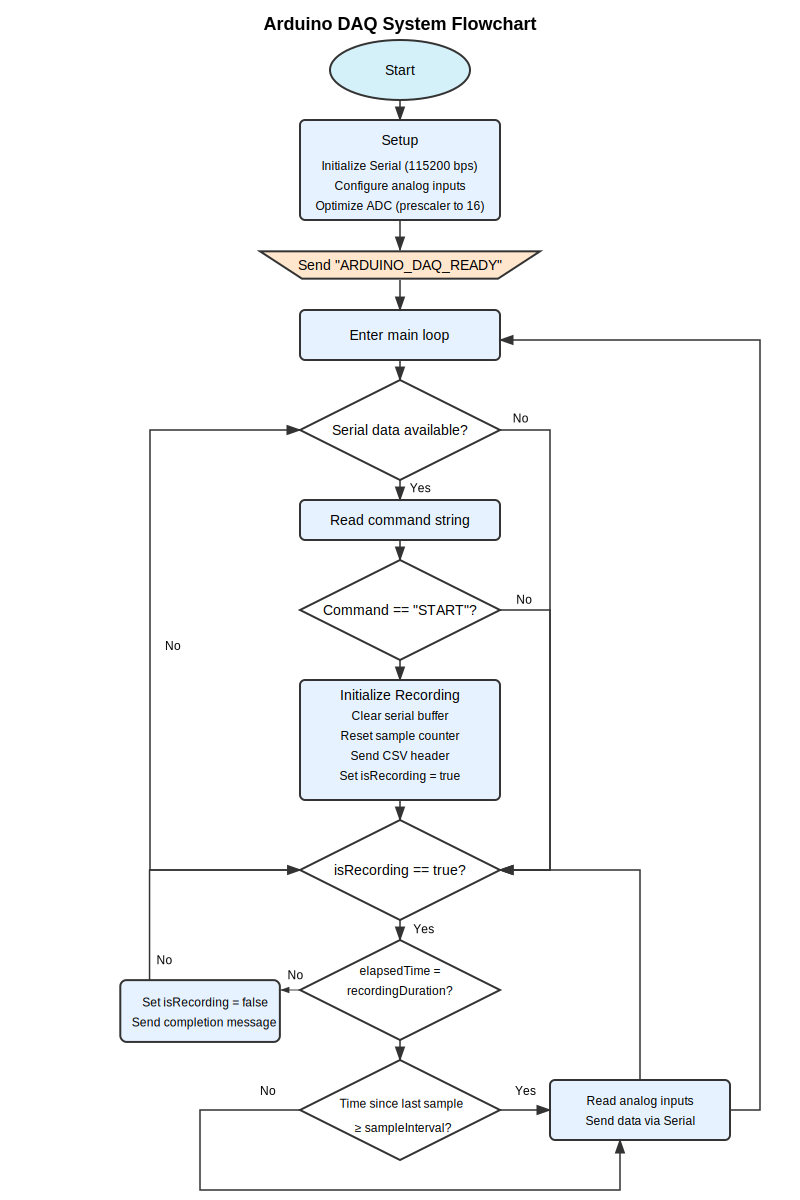
\includegraphics[width=0.6\textwidth]{chapters/methodology/ArduinoDAQ/flowchart_Arduino_code.png} % change {path}
  \caption{Flowchart of C++ code on Arduino DAQ}      
  \label{fig:daq_arduino_code}           
\end{figure}                            
\paragraph{Sampling Rate}
Several factors restrict the sampling rate:

\subparagraph{Sample Interval Setting}
The most direct limitation is the \texttt{sampleInterval} constant set to 2ms in the code, which means samples are taken no more frequently than every 2 milliseconds (500 Hz theoretical maximum).

\subparagraph{ADC Prescaler Configuration}
The ADC prescaler is set to 16 (from the default of 128) with this line:
\begin{verbatim}
ADCSRA = (ADCSRA & 0xF8) | 0x04;
\end{verbatim}
This increases the ADC clock to 16MHz/16 = 1MHz. With each conversion taking 13 ADC clock cycles, the theoretical maximum sampling rate is about 76.9kHz for a single channel.

\subparagraph{Multiple Channel Reading}
Since the system reads from 4 analog inputs sequentially, the effective per-channel sampling rate is reduced by approximately a factor of 4.

\subparagraph{Serial Transmission Overhead}
Each sample requires formatting and sending data over serial:
\begin{verbatim}
String dataString = String(sampleCount) + "," + String(elapsedTime);
// ... format and add voltage values ...
Serial.println(dataString);
\end{verbatim}
This string creation and serial transmission takes considerable time.

\subparagraph{Serial Baud Rate}
The code uses 115200 bps, which limits how quickly data can be transmitted. Each sample in this format might be around 30-40 bytes, which means \texttildelow 3000-3800 samples/second theoretical maximum throughput.

\subparagraph{String Operations}
The use of the Arduino \texttt{String} class is memory-intensive and can cause fragmentation over time, potentially causing slowdowns.

\subparagraph{Loop Cycle Time}
Other operations in the main loop consume processing time.

The dominant limiting factor in this implementation is likely the combination of the explicit 2ms sample interval and the serial communication overhead. Higher sampling rates would require optimizing the data transmission format, possibly using binary rather than text formatting, and reducing the sample interval.
